\documentclass[12pt]{article}

\usepackage{amssymb,amsmath,amsfonts,eurosym,geometry,ulem,graphicx,caption,color,setspace,sectsty,comment,footmisc,caption,natbib,pdflscape,subfigure,array,hyperref}
\usepackage{bbm, mathspec}
\usepackage{listings}
\usepackage{booktabs}
\usepackage[svgnames,table]{xcolor}
\usepackage[tableposition=above]{caption}
\usepackage{pifont}
\usepackage{float}
\usepackage{rotating}

\setcitestyle{authoryear,open={(},close={)}}

\onehalfspacing
\newtheorem{theorem}{Theorem}
\newtheorem{corollary}[theorem]{Corollary}
\newtheorem{proposition}{Proposition}
\newenvironment{proof}[1][Proof]{\noindent\textbf{#1.} }{\ \rule{0.5em}{0.5em}}

\newtheorem{hyp}{Hypothesis}
\newtheorem{assumption}{Assumption}
\newtheorem{subhyp}{Hypothesis}[hyp]
\renewcommand{\thesubhyp}{\thehyp\alph{subhyp}}

\newcommand{\red}[1]{{\color{red} #1}}
\newcommand{\blue}[1]{{\color{blue} #1}}

\newcolumntype{L}[1]{>{\raggedright\let\newline\\arraybackslash\hspace{0pt}}m{#1}}
\newcolumntype{C}[1]{>{\centering\let\newline\\arraybackslash\hspace{0pt}}m{#1}}
\newcolumntype{R}[1]{>{\raggedleft\let\newline\\arraybackslash\hspace{0pt}}m{#1}}

\geometry{left=1.0in,right=1.0in,top=1.0in,bottom=1.0in}

\definecolor{mauve}{rgb}{0.2, 0.5, 0.478}

\begin{document}
	
	\begin{titlepage}
		\title{Contract Year Effect in the NBA\thanks{We would like to thank Professor Hortaçsu and Francisco del Villar Ortiz Mena for their invaluable insights.}}
		\author{Changhao Shi\thanks{University of Chicago, The College, Economics} \and Jonathan Liu\thanks{University of Chicago, The College, Economics} \and Terry II Culpepper\thanks{University of Chicago, The College, Economics} \and Sean Choi\thanks{University of Chicago, The College, Economics}}
		\date{\today}
		\maketitle
		\begin{abstract}
			\noindent We investigate whether being in a contract year has an effect on NBA player performance, with proxies such as win shares. Data is collected with custom scrapers on basketball websites and we evaluate the underlying theory of the data and how well they serve as proxies for performance. Existing heteroskedasticity, heterogeneity of players, and correlated observations drive our approach to tackle the issues individually with an array of methods. We use an IV regression controlling for possible endogenous effects. Subsequently, we employ a generalized estimating equation on a generalized weighted OLS to tackle the issue of correlated observations in addition to the issue of heteroskedasticity and heterogeneity. We also use a double LASSO inference method to tackle the curse of dimensionality problem that we encounter along an alternate approach to solving the correlated observations problem. The results we get show that the contract year has a mildly statistically significant effect on player performance, but not on most other measures of player performance. Furthermore, we compare the three approaches and demonstrate the usefulness of tackling underlying heteroskedastic, heterogeneous, and correlated observational trends in the data for inference and statistical power. \\
			\vspace{0in}\\
			\noindent\textbf{Keywords:} Sports Economics, Athletes, Contracts, NBA\\
			\vspace{0in}\\
			\noindent\textbf{JEL Codes:} Z20, Z22 \\
			
			\bigskip
		\end{abstract}
		\setcounter{page}{0}
		\thispagestyle{empty}
	\end{titlepage}
	\pagebreak \newpage
	
	\tableofcontents
	
	\clearpage
	
	\doublespacing
	
	
	\section{Introduction} \label{sec:introduction}
	
	\subsection{Introduction and Literature Review}
	
	There has been numerous news articles highlighting the contract year phenomenon, a phenomenon where the athletes perform at a high level before their free agency than previous years, but once they sign we observe a drop in performance back to previous levels. Bismack Biyombo, Raef LaFrentz, and Luol Deng are just few of the many examples of this phenomenon. However, when watching the NBA, one finds that superstars such as Kobe Bryant, LeBron James, and Michael Jordan are not subject to the contract year phenomenon. This can be attributed to career concerns, as written by \cite{holmstrom_contracts_1999} and \cite{gibbons_1992}. Such superstars play not simply to maximize their paychecks, but also to win championships, improve their legacies, and enter the conversation for greatest player of all time. However, many other players do not face the same career concerns, and hence may simply seek to maximize paychecks for minimal effort, forming the basis of the contract year phenomenon.
	
	At its core, the contract year phenomenon is a principal-agent problem, complicated by incomplete information and time-variant incentives. In other words, a principal pays an agent, where the principal reaps utility as a function of the effort the agent puts in, while the agent reaps utility from the payment. The cost to the principal is the payment, while that to the agent is his/her effort level. Furthermore, principals are unable to observe the effort levels of agents directly, meaning that contracts offered by the principal may be incentive-incompatible. This can then lead to what \cite{alchian_1972} call "shirking" behavior, where an agent works with less effort than agreed upon in the contract. \cite{holmstrom_contracts_1999} further addresses the issue of moral hazard in a principal-agent interaction with imperfect information, and states that "[w]hen the same situation repeats itself over time, the effects of uncertainty tend to be reduced and dysfunctional behavior is more accurately revealed, thus alleviating the problem of moral hazard". However, a major issue with the contract year phenomenon is that principals, holding the expectation of high effort levels, offer long-term contracts, hence not allowing the "same situation" to play out numerous times, but only a few times before the player retires. This is intuitively suboptimal, and in fact, \cite{prendergast_1999} finds that "contracts predicted by the theory" have not been well-confirmed empirically. Thus, on the strategic level, agents on a contract year can engage in ex-ante opportunism, before undertaking ex post opportunism after signing the contract, terminology discussed in \cite{ress_1994}. Namely, agents can first exert a high level of effort in one's contract year - ex ante opportunism - which enables them to sign a long-term contract. However, after signing, the players can now act with ex post opportunism, i.e. in this case putting in minimal effort. The degree to which this effort is minimal depends on an agent's dynamic problem. In other words, they can choose to exert no effort, hence guaranteeing that they never sign a new contract again. Alternatively, they could exert some positive level of effort, such that principals will be willing to give another contract once the agent reaches his next contract year. This is within the scope of the large body of IO literature on reputation.
	
	That being said, sports-specific research has yielded conflicting results on opportunistic behavior. \cite{lehn_1982}, \cite{scoggins_1993}, \cite{stiroh_2006}, and \cite{paulsen_2018} find evidence of the aforementioned opportunistic behavior. However, \cite{krautmann_1990}, \cite{maxcy_2002}, \cite{berri_2007}, \cite{krautmann_2009} attempt to explain the differing results by arguing that the test one uses to determine shirking affects whether or not one does find such behavior. In addition, \cite{ryan_show_2015} finds that multiple studies eliminates players who fail to acquire a new contract. This creates survivorship bias, as such players are likely to have systematically lower metrics of effort in contract years, and hence coefficients estimating the contract year phenomenon may be biased upwards.
	
	Studies on the contract year phenomenon have used performance-based metrics, such as one's Player Efficiency Rating (PER, a statistic meant to measure a basketball player's per-minute performance while adjusting for the number of opportunities he has to perform), in order to estimate the impact of contract years on performance. We look at some such statistics, but instead of focusing on those, we would instead like to focus on other metrics that we believe are more closely related to effort level. This is because at the NBA level, simply exerting more effort may not be enough for many players who want to improve their performance: they face not only a talent barrier, but also a speed barrier during in-game action, where the game moves quickly and is mostly continuous. This means that the effect of effort on performance could be completely outweighed by the need to think quickly and have extremely fast reactions. This is in contrast to a sport like baseball, where a player could exert more effort by practicing his batting more, and such effort can be demonstrated relatively clearly during in-game performance due to the slow, discrete nature of the game.
	
	\subsection{Environment}
	
	Summary statistics of the environment could illuminate potential controls that we need to use for our data analysis. The first issue is that players are grouped into different positions. In general, we would expect that players play within the constraints and objectives of their positions. For example, players with position C are center will have more control over the defense, and will generally be near the basket. Owing to its position at the center, they will therefore have more opportunity to help the team's defense and so have a higher defensive win share. To make sure that our data is not skewed towards one type of player, we examine the summary statistics of our environment.
	
	\begin{figure}[H]
		\centering
		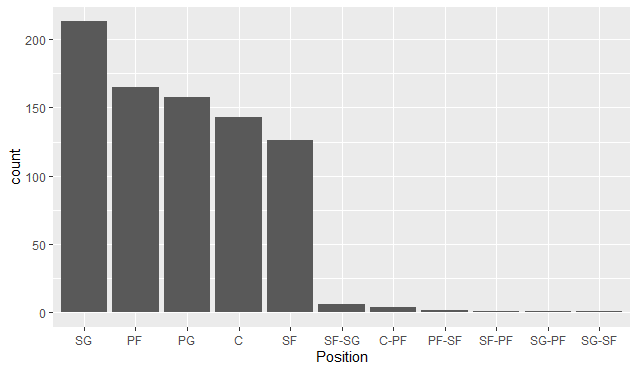
\includegraphics[width=\textwidth]{position.png}
		\caption{Position}
		\label{fig:Position}
	\end{figure}
	
	Height could also influence a player's effectiveness on the field, and taller players may gain an advantage, all else equal.
	
	\begin{figure}[H]
		\centering
		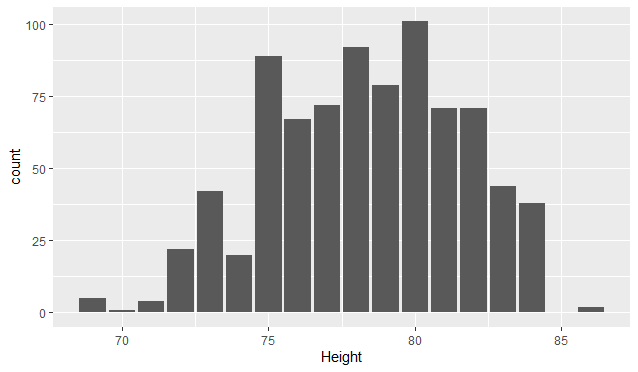
\includegraphics[width=\textwidth]{height.png}
		\caption{Height}
		\label{fig:Height}
	\end{figure}
	
	Age may impact their performance too. Because players decrease in energy over an age of 30, they may start focusing on other aspects of the game that maximizes their performance given their energy constraints, which can skew the results.
	
	\begin{figure}[H]
		\centering
		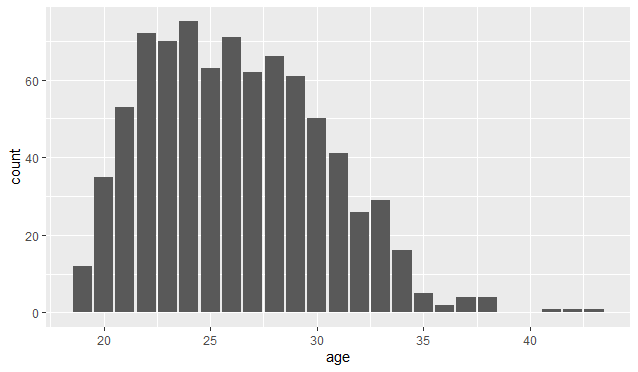
\includegraphics[width=\textwidth]{age.png}
		\caption{Age}
		\label{fig:Age}
	\end{figure}
	
	We also expect salary to correlate with the player's performance; that is, we expect, in general, that better players receive a higher salary. In the data, unfortunately we see a strong skew where a few players receive significantly higher salary than the modal salary.
	
	\begin{figure}[H]
		\centering
		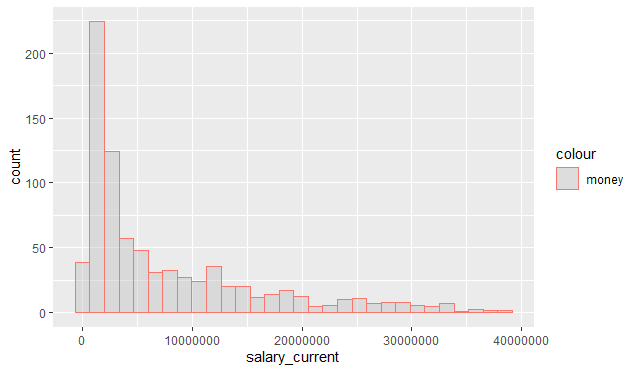
\includegraphics[width=\textwidth]{money.png}
		\caption{Salary}
		\label{fig:Salary}
	\end{figure}
	
	Finally, we will be using win shares as our main metric of evaluating performance. Note that win shares for most players cluster around 0 to 1, so a coefficient of win share that is around 0 to 1 will actually be significant; that is, a player who goes from 0 win share to 0.5 win share may literally be eclipsing 50\% of the players.	
	
	\begin{figure}[H]
		\centering
		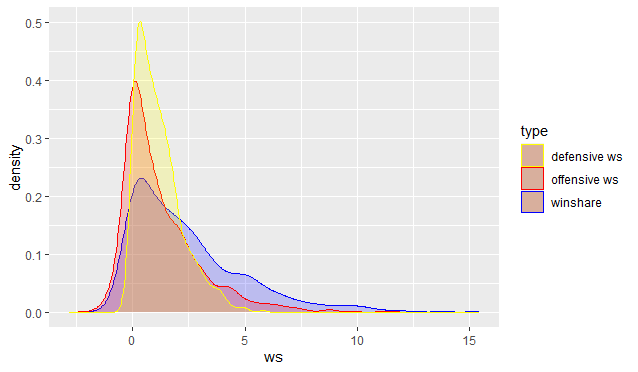
\includegraphics[width=\textwidth]{ws.png}
		\caption{Win Shares}
		\label{fig:Win Shares}
	\end{figure}	
	
	\begin{figure}[H]
		\centering
		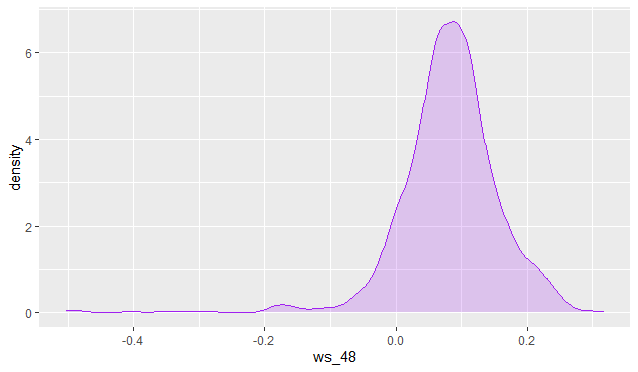
\includegraphics[width=\textwidth]{ws_48.png}
		\caption{Win Shares at 48 min.}
		\label{fig:Win Shares at 48 min.}
	\end{figure}
	
	The last relevant environmental data we require is the minutes played per game for players. Vitally, since many of the performance metrics we are using increases with minutes played (for example, the more minutes you play for your team, of course the more win shares you bring for the team), we need to control for and weight our regression by it.	
	
	\begin{figure}[H]
		\centering
		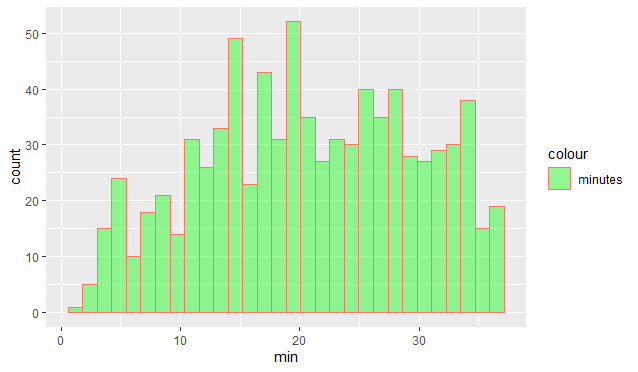
\includegraphics[width=\textwidth]{min.png}
		\caption{Minutes}
		\label{fig:Minutes}
	\end{figure}
	
	\section{Data} \label{sec:data}
	
	\subsection{Data collection}
	
	The NBA salaries of every player from the 2016-2017 season to the 2019-2020 season were collected from basketballreference.com. Note that basketballreference only displays data for the current season, so to get salary data for 2016-2017 to the 2018-2019 seasons, we utilized web.archive.org. Players were determined to be contract years if they did not have a salary for the following season. Furthermore, panel data of all advanced stats for each active NBA player was scraped from basketballreference.com for every regular season these players played in. Most of the advanced stats are measurements of a player's productivity on the court. These include the age of the player, team the player played for, position the player played for, the number of games the player played for a particular season, average minutes played per game, player efficiency rating, true shooting percentage, three-point attempt rate, free-throw attempt rate, offensive rebound percentage, defensive rebound percentage, total rebound percentage, assist percentage, free throw attempt rate, offensive rebound percentage, defensive rebound percentage, assist percentage, steal percentage, block percentage, turnover percentage, usage percentage, offensive win shares, defensive win shares, win shares, win shares per 48 minutes, offensive box plus/minus, defensive box plus/minus, box plus/minus, and value over replacement player. 
	
	Another way to measure a player's productivity/effort on the court is with boxout data. In theory, the more a player boxes out opposing players in order to grab rebounds, the more productive that player is to the team. All boxout-related data was collected from stats.nba.com for every player from the 2016-2017 to the 2019-2020 regular season. These include the number of boxouts a player averages per game, number of boxouts on offense a player averages per game, number of boxouts on defense a player averages per game, average number of rebounds the team grabs as a result of a player boxing out, average number of rebounds the player grabs as a result of him boxing out, percentage of times a player boxes out on offensive, percentage of times a player boxes out on defense, the percentage of times the teams grabs a rebound when boxing out, and the percentage of times the player grabs a rebound when boxing out. 
	
	Another method of measuring a player's value on the court is by using data on how often the player touches the ball. Players who handle the ball more often are typically much more valuable to his team. Data for player touches was collected from stats.nba.com. These include the number of touches a player averages per game, the number of touches the player averages in the front court per game, the percentage of the time the player has the ball when he is on the court, average seconds the player has the ball when he touches it, the average number of dribbles the player takes whenever he touches the ball, the number of points the player scores per touch, the average number of times a player touches the ball in the elbow part of the court, the average number of post-ups a player has per game, the average number of times a player touches the ball in the paint, points per elbow touch, points per post-up, and points per paint touch. 
	
	Note that when analyzing the data, the datasets for player salary, advanced player stats, boxouts, and touches were merged together by player name. 
	
	\subsection{Dependent variables and proxies}
	
	To analyze the impact of a player playing during a contract year on his productivity on the court, we used the following functional form:
	
	\[
	\begin{aligned}
	Production_{it} = a_1*ContractYear_{it} + a_2*Age_{it} + a_3*Minutes_{it} + a_4*Salary_{it}  \\
	+ IndividualFixedEffects + SeasonalFixedEffects + PositionFixedEffects \\
	\end{aligned}
	\]
	
	The regressions are all weighted least squares by minutes played. This is because we do not want a superstar player who averages around 40 minutes per game to be weighted the same as another NBA player who barely gets any playing time. $ContractYear$ is a variable that takes on the value of 1 if the player is playing in a contract year; 0 otherwise. $Age$ is the player's age on February 1st of the season. $Minutes$ is the average number of minutes a player averages per game. $Salary$ is the amount of money (in USD) a player is paid that season. Note that since only data from three seasons were analyzed, the effect of inflation will be marginal, at best. In addition to controlling for individual and season fixed effects, position fixed effects were also controlled for. This is because it is possible for some positions to be more valuable than others. For example, teams generally value big men/centers, so it is possible that these players can get longer contracts, so they will be less likely to be on a contract year. Furthermore, centers generally are more productive and/or valuable on the court (i.e. are responsible for grabbing many rebounds and scoring many points in the paint). 
	
	We used 16 different variables as proxies of a player's productivity: usage rate, total win shares, win shares per 48 minutes, defensive win shares, offensive win shares, average total distance moved per game (in miles), average distance moved per game on defense (in miles), average distance moved per game on offense (in miles), average speed on the court (in miles per hour), average speed on defense (in miles per hour), average speed on offense (in miles per hour), average seconds per touch, average dribbles per touch, average box outs per game, average offensive box outs per game, and average defensive box outs per game. 
	
	A few of those proxies are rather weak. For example, every measurement involving a player's speed or distance moved on the court can be extremely noisy since a player is likely not hustling all of the time. For instance, on isolation plays where an offensive player seeks to attack a defensive player one-on-one, all other players on the court are likely standing around doing nothing. This is simply due to the nature of the play where involvement from the other players is not required, not because the other players are unwilling to put in any effort. 
	
	The strongest proxies are likely the win share variables: total win shares, win shares per 48 minutes, defensive win shares, and offensive win shares. These variables are commonly used in sports analytics to measure individual performance and/or how many wins can be attributed solely to a player (https://www.basketball-reference.com/about/ws.html). For example, a player can be on a terrible team (say only wins 20 out of 82 games), but can have 15 win shares. On the other hand, a player can be on a good team (say wins 60 out of 82 games) and also have 15 win shares. Both of those players are likely just as productive and/or valuable individually. However, in the former case, the player was unable to get much help from his teammates, but in the latter case, the player was surrounded by a strong supporting cast. Note that defensive win shares is a measure of the number of wins that can be attributed solely to a player's performance on defense, and offensive win shares is a measure of the number of wins that can be attributed solely to a player's performance on offense. 
	
	\section{Model and Analysis}
	
	\subsection{Heteroskedasticity}
	
	In general, we cannot expect that the data for NBA players follows a homoskedastic trend. For example, the variance for win shares for players on a contract year can theoretically be different than the variance for offensive win shares for players not on a contract year. This is because a contract year can cause behavioral shifts that are reified in different ways: while a contract year could push one player to prioritize their win shares to impress future teams, another may feel ready to retire and gradually decrease the effort they put into each match, therefore affecting their performance. In a similar vein, we would also expect that, all else equal, players who have more time on the field to have a lower variance in performance than players who have less time on the field. An argument on the Law of Large Numbers applies here: all else equal (as in, players have the same ability and are given the same opportunities), players' performance converge to their expected performance as $t$, the time they spend on the field, goes to infinity. Heteroskedasticity in this sense may cause the OLS estimator to be unbiased but inconsistent, possibly leading to invalid inferences based on biased variances, so verifying whether the data contains underlying heteroskedasticity and tackling the problem will help with lowering the variance and therefore the precision of our results.
	
	\subsubsection{Breusch-Pagan test}
	
	We begin by looking at whether the data shows heteroskedastic trends. To do so, we use the Breusch-Pagan test from \cite{breusch_simple_1979}. Our null hypothesis is \[
	H_0:\quad x_i \text{ exhibits homoskedastic trends}
	\] for each regressor $x_i$ we are using. To do so, we assume that the variance follows a functional form $h\left(z_i'\alpha\right)$. Then, our null hypothesis would be $\alpha = 0$, where $0$ is the zero vector. Breusch and Pagan showed that this is equivalent to using the Lagrangian multiplier test statistic $\mathrm{LM}$, where \[
	\mathrm{LM} = \hat{d}' \hat{\mathcal{P}}^{-1} \hat{d}
	\] and \[
	d = \frac{\partial l}{\partial \alpha}
	\] and \[
	\mathcal{P} = -\mathbb{E}\left(\frac{\partial^2 l}{\partial\alpha \partial \alpha'}\right)
	\] and the hats are quantities that are evaluated with $\hat{\alpha}$ (\cite{breusch_simple_1979}). In $\textbf{R}$, we use the Bresuch-Pagan test on our OLS regression of win shares on contract year and our controls, and obtain a $p$-value of $6.564 \times 10^{-5}$:
	
	\lstset{frame=tb,
		language=R,
		aboveskip=3mm,
		belowskip=3mm,
		showstringspaces=false,
		columns=flexible,
		basicstyle={\small\ttfamily},
		numbers=none,
		numberstyle=\tiny\color{gray},
		keywordstyle=\color{blue},
		commentstyle=\color{dkgreen},
		stringstyle=\color{mauve},
		breaklines=true,
		breakatwhitespace=true,
		tabsize=3,
		otherkeywords = \#
	}
	
	\begin{lstlisting}
	hetero.plot <- lm(formula = ws ~ contract_year + as.factor(name) + pos + as.factor(season) +salary_current, data = nba)
	
	bptest(hetero.plot)
	\end{lstlisting}
	
	\begin{table}[H]
		\centering
		\caption{Studentized Breusch-Pagan test}
		\rowcolors{4}{}{gray!10}
		\begin{tabular}{*4c}
			\toprule
			& \multicolumn{3}{c}{Test Results} \\
			\cmidrule(lr){2-4}
			Regressand & BP  & df & p-value \\
			\midrule
			Win Shares & 501.44       & 386 & $6.564\times 10^{-5}$       \\
			Usage Rate & 580.35       & 386       & $5.266\times10^{-10}$ \\
			Boxouts & 530.19       & 386 & $1.433\times10^{-6}$ \\
			Average Speed & 548.27 & 386       & $9.901\times 10^{-8}$       \\
			Average Dribbles per Touch & 664.3  & 386 & $0$        \\
			\bottomrule
		\end{tabular}
	\end{table}
	
	The Breusch-Pagan test allows us to reject the null hypothesis that the dataset exhibits homoskedastic trends very confidently. Due to this result, we would require a method to tackle the underlying heteroskedasticity of our data.
	
	\subsubsection{Weighted OLS}
	
	A weighted OLS gives us a partial solution to this issue. Because we have reason to believe that observations of players who are given little playtime are of a worse quality than observations of players who are given plenty of playtime, a possible weighting mechanism is to use the minutes they spend per match in order to prioritize the observations of players who spend the most amount of time on the field. There is, of course, an issue of whether players who are given little playtime are different from players who are given plenty of playtime. We will turn to tackle this issue in this next section.
	
	We first note that, \emph{if} our weights are are inversely proportional to the underlying variance of the data (in other words, $W$, our weight matrix, is the inverse of the variance-covariance matrix), \emph{then} the weighted OLS estimator is the BLUE estimator (\cite{aitken_iv.least_1936}). However, there is no reason to believe that the variance \emph{is} the number of minutes in our data. Instead, it is reasonable to suppose that the variance \emph{correlates} with the number of minutes. The potential disadvantage of a weighted least squares method arises when the weights are not precise relative to one another (\cite{carroll_transformation_1988}), but because minutes played is an external measurement that is precise and are not estimated from within our data, we can be confident that the issue of weights being imprecise relative to one another is limited. To formalize our argument, we state our assumption.
	
	\begin{assumption}
		$W$, where $W$ is the weight matrix consisting of the minutes played for a given player for each observation, approximates the inverse of the variance-covariance matrix of the regression.
	\end{assumption}
	
	Our regression model is therefore \[
	y_{it} = x_{it}'\beta + \epsilon_i
	\] but we estimate $\beta$ with the weighted least square estimator \[
	\hat{\beta} = \left(X'WX\right)^{-1}X'WY
	\] where $X$ is the data matrix, $Y$ is the vector of $y_{it}$'s, and $W$ is the weight matrix. To be clear, $W$ is the matrix that consists of the minutes played for a given player for each observation, such that $X'WX$ outputs the data matrix $\hat{X}'\hat{X}$ where $\hat{X}$ consists of, for each observation $i$ and time period $t$, $w_{it}x_{it}$ This shows that we need to make the following assumption:
	
	\begin{assumption}
		$X'WX$ is an invertible matrix.
	\end{assumption}
	
	We would have to argue that we do not run into the problem of perfect multi-collinearity. This is a reasonable assumption - we do not believe, for example, that when we weight the players' age and income by the minutes played per game on the field, we obtain a linear relationship between the two. Concerns would arise if we have covariates such as total distance run and speed together. Note that these two covariates may not initially have a linear dependence, until, possibly, when we weight them by minutes played. However, we haven taken care to prevent possible multicollinearity by avoiding using covariates that have some relationship with minutes played, or may relate to another variable after being weighted by minutes played.
	
	It is easy to conduct a weighted OLS on $\textbf{R}$. We simply call the function with an additional parameter, $\textbf{weights}$, using our choice of weight, minutes played:
	
	\begin{lstlisting}
	reg.ws <- lm(formula = ws ~ contract_year + min + as.factor(name) + pos + as.factor(season) 
	+ salary_current, data = nba, weights = nba$min)
	\end{lstlisting}
	
	Finally, we use minutes played as a control once again, because the function of using minutes played as a \emph{weight} is because we think it is a good proxy for the underlying heteroskedasticity of the data, but at the same time, minutes played as a \emph{covariate} is also important as it will affect outcomes such as win shares. For instance, since win share is a measure of the amount of wins a player contributes to the team, it is natural to assume that the minutes played per match of a player will contribute to their win share. Therefore, we use minutes played as both a covariate and also the weight. We can show that the weighted OLS estimator remains unbiased if we assume that minutes played approximates the inverse of the variance-covariance matrix; however we cannot guarantee that the estimator still retains properties such as the BLUE property. We state this as a proposition:
	
	\begin{proposition}
		The weighted OLS estimator for a regression with $w_i$ as both the weight and a covariate is unbiased, but not necessarily BLUE.
	\end{proposition}
	
	A trade-off exists here: it is clear that data from players who have low minutes played should not be weighted as heavily as data from players who have high minutes played. The solution of using a weighted OLS partially tackles the problem of the underlying heteroskedasticity, which prevents the OLS estimator from being BLUE. However, because of the necessity of using minutes played as a control as well, we are forced to use a weighted OLS estimator that is not BLUE. In essence, we are choosing between the lesser of two evils here. We believe that the weighted least squares approach is the superior one because the quality of the variance contributed by players with very low minutes played is unduly large, and the deviation from efficiency of the weighted OLS estimator with the weight as a control should be lower than the deviation from efficiency of the unweighted OLS estimator which puts undue weight on low quality data.
	
	\subsection{Heterogeneity}
	
	Player performance cannot be directly observed, and existing metrics such as distance covered on the field per minute may only be loosely correlated with player performance. For example, a player may specialize in 3-point throws and so roughly run the same amount of distance but attempt more 3-point shots per game. Another player may perform by running longer each game to gain tactical advantage on a field. It is also possible that the player's performance fails to translate into an observable metric; for example, he might put in effort into team-building exercises and coordinate much more on the field.
	
	What is even worse is that the qualities of the players we have discussed that produces this heterogeneity cannot be observed. For example, their preferred playstyle, their cooperative attitude, and so on, are not something that we can observe in our data. These omitted variables, or rather, omitted fixed effects, that exhibit heterogeneity are therefore something we need to control for.
	
	To control for fixed effects, we add indicator variables for players or teams as a covariate. This, along with the existing controls, gives us the regression model \[
	y_{it} = \sum_{j=1}^N \alpha_j \mathbbm{1}\left\lbrace i= j \right\rbrace + \mathbbm{1}\left\lbrace i_t\in \mathrm{Contract} \right\rbrace\beta + c_{it}'\gamma + u_{it}
	\] where $y_{it}$ is the outcome player statistics for player $i$ in time period $t$, $\mathbbm{1}\left\lbrace i= j \right\rbrace$ is the indicator variable for players, $\mathbbm{1}\left\lbrace i_t\in \mathrm{Contract} \right\rbrace$ is the indicator variable for whether a player is in a contract year in a given time period, and $c_{it}$ are various controls, such as age and current salary. The identifying assumption is then that unobservable effects soaked up by the individual indicator variable that simultaneously affect the outcome player statistics and the explanatory variable and covariates are time-invariant. In other words, \[
	\mathrm{Cov}\left(x_{i1}, u_{it}\right) = \dots = \mathrm{Cov}\left(x_{iT}, u_{it}\right) = 0,
	\] where $x$ includes both the explanatory variable and the controls. This assumption is innocuous enough in this context. We don't expect unobserved characteristics (omitted variables) of an individual to change dramatically across years that also affect whether a given player is in a contract year. For example, a player may get married and be very happy that year. This would cause him to play better, therefore increasing his performance and we will see a change in his player statistics. However it is unlikely that it will affect whether he is in a given contract year, as that aspect largely depends on how many years ago the player signed the contract.
	
	The implementation in $\textbf{R}$ is straightforward. We simply add a dummy variable for the player's name.
	
	\begin{lstlisting}
	reg.ws <- lm(formula = ws ~ contract_year + min + as.factor(name) + pos + as.factor(season) 
	+ salary_current, data = nba, weights = nba$min)
	\end{lstlisting}
	
	\subsection{Correlated observations and within team (cluster) dependence}
	
	The performance put in by a particular player may also correlate with other players' performance. Since basketball is a team game, effort or performance put in by one player may synergize with effort or performance put in by other players. In general we expect observations to correlate strongly within-team.
	
	Let us start by examining how effort could correlate between observations. We can look at this issue game-theoretically. Consider the standard public goods game, and let $y_i$ be the energy of the player $i$ devoted to the match, out of a total of $1$ endowed unit of energy. The payoff function for player $i$ can be thought of as \[
	\Pi_i = \left(1 - y_i\right) + \alpha \sum_{j} y_j
	\] where $0<\alpha<1$. The payoff here could represent the probability of winning a match. The sum of the players' effort correlates positively with the expected probability of winning a match. When $\alpha<1$, the Nash equilibrium of this game is for all players to invest $0$ energy into the match. However, when factoring in social norms, we expect players to fall into two categories. Based on empirical evidence, players will either put in more of their endowment when others put in more, or put in less when others put in more \citep{dong_dynamics_2016}. This stylized game theoretical model and the empirical or experimental outcomes of human behavior shows that correlated observations with respect to effort is a significant issue that we need to address.
	
	Furthermore, performance could also correlate between observations. For example, win share is a metric that estimates the contribution of a player to their \emph{team}. While the win share of all players of a team does not exactly necessarily add up to the number of wins of a team (there is some more nuance than this), it does so approximately, which means that my increase in win share, all else equal, is your decrease in win share.
	
	This makes estimating the contract year effect more difficult, as the outcome variable of an individual correlates with that of other individuals. Furthermore, this correlation is ex-ante unknown. While we may have some idea of the direction of the correlation, having some precise sense of its magnitude is difficult.
	
	The first issue with correlated observations is that the OLS estimator is no longer efficient, and once again, loses the BLUE property. The second issue builds on the first, which is, once again, that an undue loss in statistical power can lead to bad inference results. The final issue is that we have very little intuition as to a possible functional form for the correlation between our outcomes.
	
	\subsubsection{Generalized estimating equation}
	
	\cite{liang_longitudinal_1986} studied an extension of generalized linear models and introduced a class of estimating equations that give consistent estimates of regression parameters and their variance even under observations with unknown correlations. We use this method as one of our approaches in tackling the issue of correlated observations. However, we will require an assumption.
	
	\begin{assumption}
		Repeated observations for a subject are independent.
	\end{assumption}
	
	The assumption is crucial for the generalized estimating equation method. We argue that this is a somewhat reasonable assumption. Since each season is independent of the previous season because the team performance in the previous season has no bearing on the initial conditions of the current season. For example, the winning team in 2017 does not get any innate advantage (in terms of competition) in 2018. While we obviously do not expect that player performance is completely independent of previous season performance (for example, the player could improve and learn from previous season mistakes), what is key is that the time dependence underlying our model is small enough and also not of key interest to our study of the contract year effect. Furthermore, we stress that, since we're attempting to correct for correlated observations that we believe is most prominent within-cluster, i.e., within-team. Hence, the \emph{subject} in the assumption is emphatically the \emph{team}, not the \emph{player}. Hence, even if player performance is not completely independent, we have good reason to assume that team performance can be approximated as independent across observations. The estimating equation is then \[
	U\left(\beta\right) = \sum_{i=1}^N \frac{\partial \mu_{it}}{\partial \beta_k} V_i^{-1} \left(Y_i - \mu_i\left(\beta\right)\right)
	\] where $\mu_{it}$ is the model mean for team $i$ at year $t$, $V_i$ is the variance-covariance matrix, and $\beta_k$ are parameters estimated by the GEE method \citep{diggle_analysis_2002}. We then use the GEE method to re-estimate our weighted OLS model, this time using team as the \textbf{cluster} we're controlling for. The code implementation in \textbf{R} is straightforward:
	
	\begin{lstlisting}
	nba <- nba %>%
	arrange(team)
	
	gee.ws <- geeglm(formula = ws ~ contract_year + min + as.factor(name) + pos + as.factor(season) 
	+ salary_current,
	family = gaussian,
	data = nba,
	weights = nba$min,
	id = team)
	\end{lstlisting}
	
	With this GEE method applied onto our weighted least squares model, we are finally able to correct for the three main challenges that we have discussed: heterogeneity, heteroskedasticity, and correlated observations.
	
	\subsection{IV Strategy}
	There is potential endogeneity bias between the outcome variable and the contract year dummy variable. Namely, not only could being on a contract year affect a player’s outcome stats, but a player’s outcome stats could affect whether a player is on a contract year. For example, a worse player may be given shorter-term contracts, since general managers would be less inclined to keep him on the roster in the long-run, meaning he is more likely to be in a contract year in general. As such, to solve this we would like an instrument that affects whether or not one is in a contract year in the current year, but has no direct effect on a player’s outcome variables.
	
	To do this, we consider the effect of LeBron James’ free agency decisions. LeBron James is a superstar in contention for the greatest player of all time, and as such his free agency decisions can shape the landscape of the entire NBA. For example, between 2011-2018, LeBron made the NBA Finals every year, out of the Eastern Conference, meaning that other Eastern teams and players did not simply plan as they normally would have due to his dominance. While Western entities competed and planned almost as usual, those in the East often chose to not compete, and instead “tank”; if a mid-tier team team decided that it could not compete against LeBron’s team, it would often choose to “blow it up” and plan for a future without LeBron, as opposed to trying to upgrade and face LeBron in the playoffs (for an example of this, look at the 2015 Hawks, and how they traded/let their star players go in order to quickly rebuild).
	
	As such, players and teams would plan contract years based on LeBron’s contract years. LeBron telegraphs his contract years a few years in advance, in order to let his current team know that if they do not surround him with good players, he will leave and join another one. This telegraphing enables players around the league to pin their contract years to his. The significance is as follows: once LeBron finishes the last year of his contract, teams/players go into limbo in free agency, waiting for LeBron to announce which team he is joining. As soon as LeBron decides and the details of his contract are announced, other teams and players exit limbo and agree to contracts based on LeBron’s choice. These contracts, though, are often similar to LeBron’s, so that once LeBron enters a contract year again, the process can restart. 
	
	For a player’s perspective, consider the following: a mid-tier player, currently in free agency, has only two offers: a low-paying, two-year offer from a contending team, and a high-paying, two-year offer from a bottom-tier team. He would like to win a championship; however, both teams are in the same conference as LeBron, so even if he joins the contending team, the chance is slim that they get to the NBA Finals. However, he knows that LeBron will enter a contract year in two years. As such, he chooses the high-paying offer on the bottom-tier team, then enters free agency at the same time as LeBron, where he can restart the process - and his quest for a championship - based on LeBron’s free agency decision.
	
	Thus, consider LeBron’s latest free agency: the summer of 2018. It was widely known that LeBron was going through great turmoil and conflict on his team at the time, the Cleveland Cavaliers, and hence teams and players knew he was likely to leave. Based on the above argument, we will use an indicator for whether or not one had a contract year in the 2018 season as an instrument.
	
	\textit{Relevance}: It clearly affects whether or not one is currently in a contract year.
	
	\textit{Exclusion}: It has no direct effect on a player’s outcome stats; it only affects outcomes through the contract year phenomenon.
	
	\textit{Exogeneity}: Anything that affects a player's outcome variables that was not controlled for will not be influenced by LeBron James' contract year status.
	
	Thus, this instrument provides an exogenous change in contract structure that affects contract year status.
	
	
	
	We test for instrument strength, finding that the F-Statistic is 85.207.
	
	\begin{table}[!htbp] \centering 
		\caption{Test for Instrument Strength} 
		\label{} 
		\begin{tabular}{@{\extracolsep{5pt}}lccccccc} 
			\\[-1.8ex]\hline 
			\hline \\[-1.8ex] 
			Statistic & \multicolumn{1}{c}{N} & \multicolumn{1}{c}{Mean} \\ 
			\hline \\[-1.8ex] 
			Df & 1 & 1.000   \\ 
			F & 1 & 85.207   \\ 
			Pr(\textgreater F) & 1 & 0.000  \\ 
			\hline \\[-1.8ex] 
		\end{tabular} 
	\end{table} 
	
	Thus, our instrumental variables model is as follows:
	
	\begin{align}
	y_i & = \alpha d_i + \beta x_i' + \epsilon_i\\
	d_i & = \gamma z_i' + \delta x_i' + \nu_i,
	\end{align}
	
	where $d_i$ is our endogenous regressor (in this case, whether or not one is on a contract year), $x_i$ is our vector of control variables, and $z_i$ is our instrument. We have that $\mathbb{E}[\epsilon_i x_i'] = \mathbb{E}[\epsilon_i z_i'] = \mathbb{E}[\nu_i x_i'] = \mathbb{E}[\nu_i z_i'] = 0$, but $\mathbb{E}[\epsilon_i \nu_i] = 0$, implying endogeneity bias.
	
	In this case, we only consider two sets of outcome variables: box outs and win shares. These are policy-relevant outcome variables for teams, as they provide metrics of a player's performance, and hence may lead to endogeneity bias.
	
	\subsection{Clustering data}
	
	\subsubsection{Correlated observations}
	
	An alternate approach to solving the correlated observations problem we discussed earlier is to change the unit of analysis. Instead of approaching the question from the player level, we approach it from the team level. This is different from the approach used when we employed the method of generalized estimation equation. We reshape the entire dataset, such that each observation is a team, rather than each cluster being a team. This sidesteps the assumption that we require to argue that a team needs to have independent observations over time, but the reshaping of the dataset will reduce the number of observations from 720 with 71 variables to 90 observations with 65 variables. Hence, we run into the curse of dimensionality problem. The data reshaping code in $\textbf{R}$ is as follows:
	
	\begin{lstlisting}
	# drop duplicate columns
	nba.LASSO <- nba %>%
	select(-"player_y") %>%
	select(-"season_1") %>%
	select(-"age_2")
	
	# filter teams that are TOT (meaning they were floating among teams)
	
	nba.LASSO <- nba.LASSO %>%
	filter(team != "TOT")
	
	# produce weighted mean by team
	
	nba.LASSO <- nba.LASSO %>%
	group_by(team, season) %>%
	mutate_all(funs(weighted.mean(.,min))) %>%
	summarize_all(mean)
	
	# drop columns that aren't meaningful when summed (produces NA)
	
	nba.LASSO <- nba.LASSO %>%
	select_if(~sum(!is.na(.)) > 0)
	\end{lstlisting}
	
	The curse of dimensionality problem, however, need not mean that we rapidly lose statistical power because our number of parameters in our regression model increases exponentially with the number of variables we have, since, for instance, we're not taking interaction terms with all variables. Our issue herein is a huge loss in statistical power and a corresponding huge increase in the variance of any regression we would run. That is to say, even a linear increase in our variance can be devastating when we only have 90 observations. Additionally, if we continue controlling for team fixed effects, this could get ugly very quickly.
	
	\subsubsection{Double LASSO inference selection}
	
	Our approach to tackling the curse of dimensionality problem is to employ the double LASSO-OLS and double LASSO-IV method described in \cite{urminsky_using_2016} based on \cite{belloni_high-dimensional_2014}. The double LASSO method serves as a tool for inference and inference selection by dropping spurious covariates that may not directly affect the data. However, in contrast with LASSO, we also attempt to ensure that we are not dropping covariates that have a small effect on the outcome variable despite being correlated significantly with the remaining covariates. That is, we want to ensure that we do not inadvertently introduce an omitted variable bias when selecting inference variables. We note that other methods, such as relaxed LASSO proposed by \cite{meinshausen_relaxed_2007} addresses some of the issues with only conducting a single LASSO (for example, a relaxed LASSO addresses the issue of computational complexity when the dimension of the dataset becomes very high, and also leads to a consistent variable selection under a prediction-optimal choice of the penalty parameters). However, the advantage of methods based on \cite{belloni_high-dimensional_2014}'s is that it is heteroskedasticity robust, with possibly non-Gaussian disturbances (which we have implicitly assumed in our GEE model), and therefore addresses the underlying heteroskedasticity of our dataset. Furthermore, the coefficient of the final OLS after the double inference is also consistent. However, we need one assumption.
	
	\begin{assumption}{``Approximate sparsity".}
		Only a relatively small number $s = o\left(n\right)$ of the regressors in the data are important for capturing accurately the main features of the regression function. In other words, the number of relevant regressors is much smaller than the sample size.
	\end{assumption}
	
	The assumption follows from \cite{belloni_high-dimensional_2014}, and is justified by carefully considering the covariates in our data. We don't have much reason to believe, for instance, that a player's dribbles per touch correlates so significantly with, say, the player's win share.
	
	\subsubsection{Pre-selection}
	
	Before we actually employ the double LASSO inference method, however, we need to take care not to use all our variables in the analysis, as several of them are correlated, or literally mean the same thing. For example, a player's offensive win shares is of course, highly correlated with their win shares. We have been hitherto circumspect and sidestepped the issue in our dataset by explicitly choosing our controls, but we now have to carefully look at all covariates in each regression and drop any covariates that serve as a proxy for effort or performance.
	
	\subsubsection{Double LASSO inference}
	
	We follow and outline the strategy in \cite{chernozhukov_high-dimensional_2016-1} for a double LASSO inference method we're going after. Our inference equation is \[
	y_{it} = d_{it} \alpha + x_{it}'\beta + \epsilon_{it}
	\] where $d_{it}$ is the inference variable, that is, the percentage of players on a contract year, weighted by their minutes played on the field. $x_{it}'$ are the usual covariates, and we are interested in the magnitude and direction of $\alpha$. As outlined in the previous section, since contract year could correlate with the error term even at the team level, we can also extend this approach and estimate the causal effect from the contract year effect using instrumental variables. In particular, we utilize the instrumental variables model once again \[
	\begin{aligned}
	y_{it} &= \alpha d_{it} + \beta x_{it}' + u_{it} \\
	d_{it} &= \gamma_0 z_{it} + \gamma x_{it}' + \upsilon_{it}
	\end{aligned}
	\] where $d$ is our inference variable once again, and $z_{it}$ is the one-dimensional instrument vector, whether the player was on a contract year in 2018. Since we have one instrument but many potential covariates, we have an issue of low-dimensional instrument and high-dimensional covariates. In this case, as outlined in \cite{chernozhukov_high-dimensional_2016-1}, we partial out the effect of the covariates from the inference variable $d_{it}$, the outcome variable $y_{it}$ and the instrumental variable $z_{it}$ with LASSO. Then, we use the residuals to compute the 2SLS estimator of the coefficient on the inference variable, $\alpha$. Finally, we then perform inference on $\alpha$ using the 2SLS estimator and heteroskedasticity robust standard errors.
	
	\section{Results} \label{sec:result}
	
	\subsection{Generalized estimating equation method}
	
	\subsubsection{Fixed effect weighted OLS}
	
	Before we discuss our results for the GEE method, let's first examine our results for the fixed effect weighted OLS. We run the fixed effect weighted OLS regression on 16 variables that we believe serve as a proxy for performance. While most of our results do not have statistical significance, such as in Table \ref{regboxout}, we found that the contract year effect is statistically significant when we use win shares as the outcome variable, consistent with our discussion that win shares is the best metric for evaluating performance, in Table \ref{regwinshare}.
	
	\begin{landscape}
		% Table created by stargazer v.5.2.2 by Marek Hlavac, Harvard University. E-mail: hlavac at fas.harvard.edu
		% Date and time: Fri, Jun 12, 2020 - 7:13:02 AM
		\begin{table}[!htbp] \centering 
			\caption{Using Box Outs as the Dependent Variables} 
			\label{regboxout} 
			\begin{tabular}{@{\extracolsep{5pt}}lccc} 
				\\[-1.8ex]\hline 
				\hline \\[-1.8ex] 
				& \multicolumn{3}{c}{\textit{Dependent variable:}} \\ 
				\cline{2-4} 
				\\[-1.8ex] & Defensive Box Outs & Offensive Box Outs & Box Outs \\ 
				\\[-1.8ex] & (1) & (2) & (3)\\ 
				\hline \\[-1.8ex] 
				Contract Year & 0.027 & 0.030 & 0.060 \\ 
				& ($-$0.107, 0.161) & ($-$0.036, 0.096) & ($-$0.113, 0.233) \\ 
				& p = 0.697 & p = 0.367 & p = 0.500 \\ 
				& & & \\ 
				Average Minutes Played & 0.069 & 0.012 & 0.081 \\ 
				& (0.054, 0.084) & (0.005, 0.020) & (0.062, 0.101) \\ 
				& p = 0.000$^{***}$ & p = 0.002$^{***}$ & p = 0.000$^{***}$ \\ 
				& & & \\ 
				Current Salary & 0.000 & 0.000 & 0.000 \\ 
				& ($-$0.000, 0.00000) & ($-$0.000, 0.000) & ($-$0.000, 0.00000) \\ 
				& p = 0.594 & p = 0.083$^{*}$ & p = 0.312 \\ 
				& & & \\ 
				Constant & 0.602 & $-$0.260 & 0.349 \\ 
				& ($-$0.245, 1.450) & ($-$0.677, 0.156) & ($-$0.743, 1.440) \\ 
				& p = 0.165 & p = 0.222 & p = 0.532 \\ 
				& & & \\ 
				\hline \\[-1.8ex] 
				Player Fixed Effects & Yes & Yes & Yes \\ 
				Year Fixed Effects & Yes & Yes & Yes \\ 
				Position Fixed Effects & Yes & Yes & Yes \\ 
				Observations & 820 & 820 & 820 \\ 
				R$^{2}$ & 0.913 & 0.838 & 0.912 \\ 
				Adjusted R$^{2}$ & 0.835 & 0.693 & 0.833 \\ 
				Residual Std. Error (df = 432) & 2.840 & 1.400 & 3.660 \\ 
				F Statistic (df = 387; 432) & 11.700$^{***}$ & 5.770$^{***}$ & 11.500$^{***}$ \\ 
				\hline 
				\hline \\[-1.8ex] 
				\textit{Note:}  & \multicolumn{3}{r}{$^{*}$p$<$0.1; $^{**}$p$<$0.05; $^{***}$p$<$0.01} \\ 
			\end{tabular} 
		\end{table}
		
		% Table created by stargazer v.5.2.2 by Marek Hlavac, Harvard University. E-mail: hlavac at fas.harvard.edu
		% Date and time: Fri, Jun 12, 2020 - 7:15:13 AM
		\begin{table}[!htbp] \centering 
			\caption{Using Win Shares as the Dependent Variables} 
			\label{regwinshare}
			\begin{tabular}{@{\extracolsep{5pt}}lcccc} 
				\\[-1.8ex]\hline 
				\hline \\[-1.8ex] 
				& \multicolumn{4}{c}{\textit{Dependent variable:}} \\ 
				\cline{2-5} 
				\\[-1.8ex] & Win Shares & Offensive Win Shares & Defensive Win Shares & Win Shares per 48 Minutes \\ 
				\\[-1.8ex] & (1) & (2) & (3) & (4)\\ 
				\hline \\[-1.8ex] 
				Contract Year & 0.401 & 0.282 & 0.102 & 0.003 \\ 
				& (0.083, 0.719) & (0.049, 0.515) & ($-$0.039, 0.243) & ($-$0.005, 0.011) \\ 
				& p = 0.014$^{**}$ & p = 0.019$^{**}$ & p = 0.156 & p = 0.445 \\ 
				& & & & \\ 
				Average Minutes Played & 0.164 & 0.112 & 0.052 & 0.002 \\ 
				& (0.129, 0.200) & (0.086, 0.138) & (0.036, 0.068) & (0.001, 0.003) \\ 
				& p = 0.000$^{***}$ & p = 0.000$^{***}$ & p = 0.000$^{***}$ & p = 0.0001$^{***}$ \\ 
				& & & & \\ 
				Current Salary & $-$0.00000 & $-$0.00000 & $-$0.000 & $-$0.000 \\ 
				& ($-$0.00000, 0.000) & ($-$0.00000, $-$0.000) & ($-$0.00000, 0.000) & ($-$0.000, 0.000) \\ 
				& p = 0.052$^{*}$ & p = 0.035$^{**}$ & p = 0.331 & p = 0.120 \\ 
				& & & & \\ 
				Constant & $-$0.098 & $-$1.210 & 1.160 & 0.062 \\ 
				& ($-$2.110, 1.910) & ($-$2.690, 0.261) & (0.274, 2.050) & (0.012, 0.112) \\ 
				& p = 0.924 & p = 0.108 & p = 0.011$^{**}$ & p = 0.016$^{**}$ \\ 
				& & & & \\ 
				\hline \\[-1.8ex] 
				Player Fixed Effects & Yes & Yes & Yes & Yes \\ 
				Year Fixed Effects & Yes & Yes & Yes & Yes \\ 
				Position Fixed Effects & Yes & Yes & Yes & Yes \\ 
				Observations & 820 & 820 & 820 & 820 \\ 
				R$^{2}$ & 0.863 & 0.863 & 0.813 & 0.829 \\ 
				Adjusted R$^{2}$ & 0.741 & 0.740 & 0.646 & 0.676 \\ 
				Residual Std. Error (df = 432) & 6.740 & 4.940 & 2.980 & 0.167 \\ 
				F Statistic (df = 387; 432) & 7.060$^{***}$ & 7.010$^{***}$ & 4.860$^{***}$ & 5.420$^{***}$ \\ 
				\hline 
				\hline \\[-1.8ex] 
				\textit{Note:}  & \multicolumn{4}{r}{$^{*}$p$<$0.1; $^{**}$p$<$0.05; $^{***}$p$<$0.01} \\ 
			\end{tabular} 
		\end{table}
	\end{landscape}
	
	
	\subsubsection{GEE Data}
	
	The GEE method gives us a smaller error by using the Wald statistic to compute the $p$-value and standard error. As we can see in Table \ref{geewinshare}, we are therefore able to bound the 95\% confidence interval for our coefficients further. Hence, we can see that the GEE method improves statistical significance for datasets with underlying correlated observations and improves statistical power, serving as a method to limit the presence of correlated observations from exaggerating the lack of statistical power of our results. We can see these comparisons in Tables \ref{geelmcomparison}, \ref{geelmcomparisonw}, and \ref{geelmcomparisond}.
	
	
	\begin{landscape}
		% Table created by stargazer v.5.2.2 by Marek Hlavac, Harvard University. E-mail: hlavac at fas.harvard.edu
		% Date and time: Fri, Jun 12, 2020 - 7:15:13 AM
		\begin{table}[!htbp] \centering 
			\caption{Using Win Shares as the Dependent Variables} 
			\label{geewinshare} 
			\begin{tabular}{@{\extracolsep{5pt}}lccc} 
				\\[-1.8ex]\hline 
				\hline \\[-1.8ex] 
				& \multicolumn{3}{c}{\textit{Dependent variable:}} \\ 
				\cline{2-4} 
				\\[-1.8ex] & Win Shares & Offensive Win Shares & Defensive Win Shares \\ 
				\\[-1.8ex] & (1) & (2) & (3)\\ 
				\hline \\[-1.8ex] 
				Contract Year & 0.401 & 0.282 & 0.102 \\ 
				& (0.126, 0.676) & (0.0578, 0.507) & ($-$0.0190, 0.223) \\ 
				& p = 0.0043$^{***}$ & p = 0.0137$^{**}$ & p = 0.09829$^{*}$ \\ 
				& & & \\ 
				Average Minutes Played & 0.164 & 0.112 & 0.0522 \\ 
				& (0.138, 0.191) & (0.0926, 0.131) & (0.0369, 0.0675) \\ 
				& p = 0.000$^{***}$ & p = 0.000$^{***}$ & p = 0.000$^{***}$ \\ 
				& & & \\ 
				Current Salary & 0.000 & 0.000 & 0.000 \\ 
				& ($-$0.000, 0.000) & ($-$0.000, 0.000) & ($-$0.000, 0.00000) \\ 
				& p = 0.163 & p = 0.0801$^{*}$ & p = 0.524 \\ 
				& & & \\ 
				Constant & -0.0984 & $-$1.21 & 1.16 \\ 
				& ($-$1.56, 1.36) & ($-$2.11, $-$0.316) & (0.344, 1.98) \\ 
				& p = 0.895 & p = 0.0081 & p = 0.005$^{***}$ \\ 
				& & & \\ 
				\hline \\[-1.8ex] 
				Player Fixed Effects & Yes & Yes & Yes \\ 
				Year Fixed Effects & Yes & Yes & Yes \\ 
				Position Fixed Effects & Yes & Yes & Yes \\ 
				Number of Clusters & 31 & 31 & 31 \\ 
				Maximum Cluster Size & 114 & 114 & 114 \\ 
				Degrees of Freedom & 820 & 820 & 820 \\ 
				Residual Degrees of Freedom & 432 & 432 & 432 \\ 
				\hline 
				\hline \\[-1.8ex] 
				\textit{Note:}  & \multicolumn{3}{r}{$^{*}$p$<$0.1; $^{**}$p$<$0.05; $^{***}$p$<$0.01} \\ 
			\end{tabular} 
		\end{table}
	\end{landscape}
	
	\begin{table}[!htbp]
		\centering
		\caption{Comparison of regression results with or without GEE for win shares}
		\label{geelmcomparison} 
		\rowcolors{4}{}{gray!10}
		\begin{tabular}{*4c}
			\toprule
			& \multicolumn{3}{c}{Relevant Statistics from weighted least squares} \\
			\cmidrule(lr){2-4}
			Coefficient/GEE & Coefficient  & Confidence Interval (95) & $p$-value \\
			\midrule
			Regular WOLS, Contract Year & 0.401       & (0.083, 0.719) & $0.014^{**}$       \\
			WOLS with GEE, Contract Year & 0.401      & (0.126, 0.676)       & $0.0043^{***}$ \\
			Regular WOLS, Minutes Played & 0.164       & (0.129, 0.200) & $0.000^{***}$ \\
			WOLS with GEE, Minutes Played & 0.164 & (0.138, 0.191)       & $0.000^{***}$       \\
			\bottomrule
		\end{tabular}
	\end{table}
	
	\begin{table}[!htbp]
		\centering
		\caption{Comparison of regression results with or without GEE for offensive win shares}
		\label{geelmcomparisonw} 
		\rowcolors{4}{}{gray!10}
		\begin{tabular}{*4c}
			\toprule
			& \multicolumn{3}{c}{Relevant Statistics from weighted least squares} \\
			\cmidrule(lr){2-4}
			Coefficient/GEE & Coefficient  & Confidence Interval (95) & $p$-value \\
			\midrule
			Regular WOLS, Contract Year & 0.282       & (0.049, 0.515) & $0.019^{**}$       \\
			WOLS with GEE, Contract Year & 0.282      & (0.0578, 0.507)       & $0.0137^{**}$ \\
			Regular WOLS, Minutes Played & 0.112       & (0.086, 0.138) & $0.000^{***}$ \\
			WOLS with GEE, Minutes Played & 0.112 & (0.0926, 0.131)       & $0.000^{***}$       \\
			\bottomrule
		\end{tabular}
	\end{table}
	
	\begin{table}[!htbp]
		\centering
		\caption{Comparison of regression results with or without GEE for defensive win shares}
		\label{geelmcomparisond} 
		\rowcolors{4}{}{gray!10}
		\begin{tabular}{*4c}
			\toprule
			& \multicolumn{3}{c}{Relevant Statistics from weighted least squares} \\
			\cmidrule(lr){2-4}
			Coefficient/GEE & Coefficient  & Confidence Interval (95) & $p$-value \\
			\midrule
			Regular WOLS, Contract Year & 0.102       & ($-$0.039, 0.243) & $0.156$       \\
			WOLS with GEE, Contract Year & 0.102      & ($-$0.0190, 0.223)       & $0.09829^{*}$ \\
			Regular WOLS, Minutes Played & 0.0522       & (0.036, 0.068) & $0.000^{***}$ \\
			WOLS with GEE, Minutes Played & 0.0522 & (0.0369, 0.0675)       & $0.000^{***}$       \\
			\bottomrule
		\end{tabular}
	\end{table}
	
	Additional tables and plots from the weighted OLS regression are presented in the appendix (\ref{sec:tab}).
	
	\pagebreak
	
	\subsection{Instrumental variable method}
	
	In the IV method, we do not find any significant results. However, the IV regression gives us a large increase in the effect of a contract year on defensive win shares and total win shares, as opposed to the standard fixed effects regression. 
	
	\begin{table}[!htbp] \centering 
		\caption{IV with Box Outs as the Dependent Variable} 
		\label{} 
		\begin{tabular}{@{\extracolsep{5pt}}lccc} 
			\\[-1.8ex]\hline 
			\hline \\[-1.8ex] 
			& \multicolumn{3}{c}{\textit{Dependent variable:}} \\ 
			\cline{2-4} 
			\\[-1.8ex] & \multicolumn{3}{c}{Box Out Metrics} \\ 
			\\[-1.8ex] & Defensive Box Outs & Offensive Box Outs & Total Box Outs\\ 
			\hline \\[-1.8ex] 
			Contract Year & 10.407 & 1.384 & 6.731 \\ 
			& (11.072) & (1.058) & (5.391) \\ 
			& & & \\ 
			Current Salary & 0.00000 & 0.00000 & 0.00000 \\ 
			& (0.00000) & (0.00000) & (0.00000) \\ 
			& & & \\ 
			Average Minutes Played & 0.184 & 0.023$^{*}$ & 0.137$^{**}$ \\ 
			& (0.134) & (0.012) & (0.060) \\ 
			& & & \\ 
			Age & $-$1.386 & $-$0.266$^{**}$ & $-$1.186$^{**}$ \\ 
			& (1.117) & (0.108) & (0.524) \\ 
			& & & \\ 
			Constant & 20.805 & 3.832$^{**}$ & 17.835$^{**}$ \\ 
			& (16.143) & (1.511) & (7.149) \\ 
			& & & \\ 
			\hline \\[-1.8ex] 
			\hline 
			\hline \\[-1.8ex] 
			\textit{Note:}  & \multicolumn{3}{r}{$^{*}$p$<$0.1; $^{**}$p$<$0.05; $^{***}$p$<$0.01} \\ 
		\end{tabular} 
	\end{table} 
	
	\begin{table}[!htbp] \centering 
		\caption{IV with Win Shares as the Dependent Variable} 
		\label{} 
		\begin{tabular}{@{\extracolsep{5pt}}lcccc} 
			\\[-1.8ex]\hline 
			\hline \\[-1.8ex] 
			& \multicolumn{4}{c}{\textit{Dependent variable:}} \\ 
			\cline{2-5} 
			\\[-1.8ex] & \multicolumn{4}{c}{Win Share Metrics} \\ 
			\\[-1.8ex] & Defensive WS & Offensive WS & Total WS & WS Per 48 Minutes\\ 
			\hline \\[-1.8ex] 
			Contract Year & 4.273 & $-$0.457 & 3.719 & $-$0.169 \\ 
			& (3.700) & (1.524) & (3.948) & (0.145) \\ 
			& & & & \\ 
			Current Salary & 0.00000 & $-$0.00000 & 0.00000 & $-$0.000 \\ 
			& (0.00000) & (0.00000) & (0.00000) & (0.000) \\ 
			& & & & \\ 
			Average Minutes Played & 0.094$^{**}$ & 0.102$^{***}$ & 0.194$^{***}$ & 0.0005 \\ 
			& (0.040) & (0.019) & (0.042) & (0.002) \\ 
			& & & & \\ 
			Age & $-$0.536 & $-$0.182 & $-$0.708$^{*}$ & 0.012 \\ 
			& (0.358) & (0.162) & (0.378) & (0.014) \\ 
			& & & & \\ 
			Constant & 6.682 & 2.862 & 9.561$^{*}$ & $-$0.011 \\ 
			& (4.817) & (2.305) & (5.103) & (0.190) \\ 
			& & & & \\ 
			\hline \\[-1.8ex] 
			\hline 
			\hline \\[-1.8ex] 
			\textit{Note:}  & \multicolumn{4}{r}{$^{*}$p$<$0.1; $^{**}$p$<$0.05; $^{***}$p$<$0.01} \\ 
		\end{tabular} 
	\end{table} 
	
	\subsection{Clustered data double LASSO inference method}
	
	\subsubsection{Double LASSO without instruments}
	
	The clustered data method when we do not utilize instruments ultimately did not lead to statistically significant results, despite ultimately only controlling on three covariates: contract year, age, and minutes played. That the number of observations was severely limited, being at 90, was a possible factor in why we could not get statistically significant results.
	
	\begin{table}[!htbp]
		\centering
		\caption{Double LASSO inference method with win share as the outcome variable}
		\label{lassows} 
		\rowcolors{4}{}{gray!10}
		\begin{tabular}{*4c}
			\toprule
			& \multicolumn{3}{c}{Relevant Statistics from double LASSO} \\
			\cmidrule(lr){2-4}
			Variable & Coefficient  & Confidence Interval (95) & $p$-value \\
			\midrule
			Contract Year & 0.990       & ($-$0.902, 2.88) & $0.31$       \\
			\bottomrule
			\textit{Note:}  & \multicolumn{3}{r}{Selected covariates: Age, Minutes Played} \\ 
		\end{tabular}
	\end{table}
	
	\begin{table}[!htbp]
		\centering
		\caption{Double LASSO inference method with offensive win share as the outcome variable}
		\label{lassoows} 
		\rowcolors{4}{}{gray!10}
		\begin{tabular}{*4c}
			\toprule
			& \multicolumn{3}{c}{Relevant Statistics from double LASSO} \\
			\cmidrule(lr){2-4}
			Variable & Coefficient  & Confidence Interval (95) & $p$-value \\
			\midrule
			Contract Year & 0.865       & ($-$0.34, 2.07) & $0.16$       \\
			\bottomrule
			\textit{Note:}  & \multicolumn{3}{r}{Selected covariates: Age, Minutes Played} \\
		\end{tabular}
	\end{table}
	
	\begin{table}[!htbp]
		\centering
		\caption{Double LASSO inference method with defensive win share as the outcome variable}
		\label{lassodws} 
		\rowcolors{4}{}{gray!10}
		\begin{tabular}{*4c}
			\toprule
			& \multicolumn{3}{c}{Relevant Statistics from double LASSO} \\
			\cmidrule(lr){2-4}
			Variable & Coefficient  & Confidence Interval (95) & $p$-value \\
			\midrule
			Contract Year & 0.0227       & ($-$0.956, 1) & $0.96$       \\
			\bottomrule
			\textit{Note:}  & \multicolumn{3}{r}{Selected covariates: None} \\
		\end{tabular}
	\end{table}
	
	\subsubsection{Double LASSO with instruments}
	
	Surprisingly, with the clustered data, and utilizing the instruments we identified during the 2SLS estimation, double LASSO works pretty well and lead to statistically significant results, although this statistical significance is still of a \emph{slightly} lesser degree than that of the GEE weighted least squares approach for win shares, but this statistical significance is of a \emph{slightly} higher degree when it comes to defensive win shares. We compare the two approaches in Table \ref{lassoivvsgee}. The magnitude of the coefficient matters here: with a regular WOLS, we do not correct for the endogenous effect, so the effect is underestimated. Consequently, for regressions where the coefficient gets close to zero, we start to lose statistical power because the confidence interval will start to overlap $0$. However, when we correct for the endogeneity bias with instruments, the coefficient is no longer underestimated in magnitude and increases drastically in magnitude. Hence, even if the error resulting from the curse of dimensionality and the low number of observations is fairly substantial, and even if the magnitude of the confidence interval is fairly high, because the coefficient is further away from zero, our statistical power also gets better. That does not mean, however, the curse of dimensionality faded from existence. It has merely shifted to the problem of the magnitude of the contract year effect being ambiguous. For instance, the 95\% confidence interval for the contract year effect on win share is (2.65, 18.1). It is quite hard to say exactly how strong the contract year effect. We can only demonstrate that the contract year effect exists.
	
	\begin{table}[!htbp]
		\centering
		\caption{Double LASSO with instruments with win share as the outcome variable}
		\label{lassoivws} 
		\rowcolors{4}{}{gray!10}
		\begin{tabular}{*4c}
			\toprule
			& \multicolumn{3}{c}{Relevant Statistics from double LASSO} \\
			\cmidrule(lr){2-4}
			Variable & Coefficient  & Confidence Interval (95) & $p$-value \\
			\midrule
			Contract Year & 10.38       & (2.65, 18.1) & $0.0085$       \\
			\bottomrule
			\textit{Note:}  & \multicolumn{3}{r}{Selected covariates: Age, Minutes Played} \\ 
		\end{tabular}
	\end{table}
	
	\begin{table}[!htbp]
		\centering
		\caption{Double LASSO with instruments with offensive win share as the outcome variable}
		\label{lassoivows} 
		\rowcolors{4}{}{gray!10}
		\begin{tabular}{*4c}
			\toprule
			& \multicolumn{3}{c}{Relevant Statistics from double LASSO} \\
			\cmidrule(lr){2-4}
			Variable & Coefficient  & Confidence Interval (95) & $p$-value \\
			\midrule
			Contract Year & 5.54       & (1.17, 9.91) & $0.013$       \\
			\bottomrule
			\textit{Note:}  & \multicolumn{3}{r}{Selected covariates: Age, Minutes Played} \\
		\end{tabular}
	\end{table}
	
	\begin{table}[!htbp]
		\centering
		\caption{Double LASSO with instruments with defensive win share as the outcome variable}
		\label{lassoivdws} 
		\rowcolors{4}{}{gray!10}
		\begin{tabular}{*4c}
			\toprule
			& \multicolumn{3}{c}{Relevant Statistics from double LASSO} \\
			\cmidrule(lr){2-4}
			Variable & Coefficient  & Confidence Interval (95) & $p$-value \\
			\midrule
			Contract Year & 5.86       & (1.22, 10.5) & $0.013$       \\
			\bottomrule
			\textit{Note:}  & \multicolumn{3}{r}{Selected covariates: Age, Minutes Played} \\
		\end{tabular}
	\end{table}
	
	\begin{landscape}
		\begin{table}[!htbp]
			\centering
			\caption{Comparison between double LASSO with instruments and weighted OLS with GEE}
			\label{lassoivvsgee} 
			\rowcolors{4}{}{gray!10}
			\begin{tabular}{*4c}
				\toprule
				& \multicolumn{3}{c}{Relevant Statistics} \\
				\cmidrule(lr){2-4}
				Variable & Coefficient  & Confidence Interval (95) & $p$-value \\
				\midrule
				Win Shares: WOLS with GEE, Contract Year & 0.401       & (0.126, 0.675) & $0.0043$       \\
				Win Shares: Double LASSO with instruments, Contract Year & 10.38       & (2.65, 18.1) & $0.0085$       \\
				Offensive WS: WOLS with GEE, Contract Year & 0.282       & (0.0578, 0.507) & $0.0137$       \\
				Offensive WS: Double LASSO with instruments, Contract Year & 5.54       & (1.17, 9.91) & $0.013$       \\
				Defensive WS: WOLS with GEE, Contract Year & 0.102       & ($-$0.0190, 0.223) & $0.09829$       \\
				Defensive WS: Double LASSO with instruments, Contract Year & 5.86       & (1.22, 10.5) & $0.013$       \\
				\bottomrule
				\textit{Note:}  & \multicolumn{3}{r}{Selected covariates: Age, Minutes Played} \\
			\end{tabular}
		\end{table}
	\end{landscape}
	
	\pagebreak
	
	\section{Discussions} \label{sec:discussion}
	
	\section{Conclusion} \label{sec:conclusion}
	
	Overall, we find that being on a contract year marginally, at best, increases an NBA player's production on the court. When running weighted least squares, while the effect of being on the contract year was not significant for most of the proxies for player production, the effect was significantly positive when using win shares and offensive win shares as the dependent variable. Surprisingly, the effect of contract year was much less significant when using defensive win shares as the proxy. This can indicate that players on contract years tend to perform better offensively. One possibility is that players on contract years feel more pressured to make an impact on the offensive end than the defensive end of the court. Perhaps it is much easier to notice a player's efforts on offense than on defense. After all, it is very easy to see if scoring more often and/or facilitating the offense directly leading to buckets. However, it might be difficult to notice a player playing better defense. For example, it is possible for opposing players to score despite solid defense. In those instances, it is much easier to notice the brilliant offense as opposed to the strong defense. As a result, when players are on the final year of their contracts, they decide to give much more effort on offense as opposed to on defense. 
	
	When using being on a contract year in 2018 as an instrumental variable for being on a contract year, the contract-year effect was found not to be significant, even when using win shares as the dependent variable. However, when employing the double lasso method while using the same instrumental variable, the contract-year effect was found to be significant when using win shares, offensive win shares, and defensive win shares as proxies for player production. But, when using the double lasso method without the instrumental variable, the contract-year effect was again found not to be significant when using any of the win shares variables as proxies for player production. 
	
	Thus, the results indicate that the fact that a player is on a contract year provides a mild, if any, boost to his production on the court. The production boost is more heavily weighted towards the offensive end as opposed to the defensive end. Further research topics include seeing if the same results hold in other professional basketball leagues. It would also be interesting to see if similar results hold in other professional sports such as baseball, football, and soccer. 
	
	\clearpage
	
	
	\clearpage
	
	\singlespacing
	\bibliographystyle{abbrvnat}
	\bibliography{citation}
	
	
	
	\clearpage
	
	\onehalfspacing
	
	\appendix
	
	\section{Tables} \label{sec:tab}
	
	We present all tables for our regression results in this section.
	
	\begin{landscape}
		% Table created by stargazer v.5.2.2 by Marek Hlavac, Harvard University. E-mail: hlavac at fas.harvard.edu
		% Date and time: Fri, Jun 12, 2020 - 7:22:29 AM
		\begin{table}[!htbp] \centering 
			\caption{Using Speed Metrics as the Dependent Variable} 
			\label{} 
			\begin{tabular}{@{\extracolsep{5pt}}lccc} 
				\\[-1.8ex]\hline 
				\hline \\[-1.8ex] 
				& \multicolumn{3}{c}{\textit{Dependent variable:}} \\ 
				\cline{2-4} 
				\\[-1.8ex] & Average Speed & Offensive Speed & Defensive Speed \\ 
				\\[-1.8ex] & (1) & (2) & (3)\\ 
				\hline \\[-1.8ex] 
				Contract Year & $-$0.006 & $-$0.009 & $-$0.009 \\ 
				& ($-$0.022, 0.011) & ($-$0.038, 0.021) & ($-$0.031, 0.014) \\ 
				& p = 0.502 & p = 0.555 & p = 0.444 \\ 
				& & & \\ 
				Average Minutes Played & $-$0.005 & $-$0.005 & $-$0.007 \\ 
				& ($-$0.007, $-$0.003) & ($-$0.009, $-$0.002) & ($-$0.010, $-$0.005) \\ 
				& p = 0.00000$^{***}$ & p = 0.002$^{***}$ & p = 0.00000$^{***}$ \\ 
				& & & \\ 
				Current Salary & 0.000 & 0.000 & $-$0.000 \\ 
				& ($-$0.000, 0.000) & ($-$0.000, 0.000) & ($-$0.000, $-$0.000) \\ 
				& p = 0.716 & p = 0.506 & p = 0.006$^{***}$ \\ 
				& & & \\ 
				Constant & 4.590 & 5.070 & 4.220 \\ 
				& (4.490, 4.700) & (4.890, 5.260) & (4.080, 4.360) \\ 
				& p = 0.000$^{***}$ & p = 0.000$^{***}$ & p = 0.000$^{***}$ \\ 
				& & & \\ 
				\hline \\[-1.8ex] 
				Player Fixed Effects & Yes & Yes & Yes \\ 
				Year Fixed Effects & Yes & Yes & Yes \\ 
				Position Fixed Effects & Yes & Yes & Yes \\ 
				Observations & 820 & 820 & 820 \\ 
				R$^{2}$ & 0.936 & 0.872 & 0.898 \\ 
				Adjusted R$^{2}$ & 0.880 & 0.758 & 0.806 \\ 
				Residual Std. Error (df = 432) & 0.351 & 0.625 & 0.472 \\ 
				F Statistic (df = 387; 432) & 16.500$^{***}$ & 7.630$^{***}$ & 9.780$^{***}$ \\ 
				\hline 
				\hline \\[-1.8ex] 
				\textit{Note:}  & \multicolumn{3}{r}{$^{*}$p$<$0.1; $^{**}$p$<$0.05; $^{***}$p$<$0.01} \\ 
			\end{tabular} 
		\end{table} 
		
		% Table created by stargazer v.5.2.2 by Marek Hlavac, Harvard University. E-mail: hlavac at fas.harvard.edu
		% Date and time: Fri, Jun 12, 2020 - 7:23:55 AM
		\begin{table}[!htbp] \centering 
			\caption{Using Distance as the Dependent Variable} 
			\label{} 
			\begin{tabular}{@{\extracolsep{5pt}}lccc} 
				\\[-1.8ex]\hline 
				\hline \\[-1.8ex] 
				& \multicolumn{3}{c}{\textit{Dependent variable:}} \\ 
				\cline{2-4} 
				\\[-1.8ex] & Distance: Defensive & Distance: Offensive & Distance \\ 
				\\[-1.8ex] & (1) & (2) & (3)\\ 
				\hline \\[-1.8ex] 
				Contract Year & $-$0.004 & $-$0.001 & $-$24.800 \\ 
				& ($-$0.009, 0.002) & ($-$0.008, 0.005) & ($-$72.200, 22.500) \\ 
				& p = 0.183 & p = 0.722 & p = 0.305 \\ 
				& & & \\ 
				Average Minutes Played & 0.033 & 0.039 & 379.000 \\ 
				& (0.032, 0.034) & (0.038, 0.039) & (373.000, 384.000) \\ 
				& p = 0.000$^{***}$ & p = 0.000$^{***}$ & p = 0.000$^{***}$ \\ 
				& & & \\ 
				Current Salary & $-$0.000 & 0.000 & 0.00000 \\ 
				& ($-$0.000, 0.000) & (0.000, 0.000) & ($-$0.00000, 0.00001) \\ 
				& p = 0.233 & p = 0.002$^{***}$ & p = 0.095$^{*}$ \\ 
				& & & \\ 
				Constant & $-$0.0003 & 0.057 & 291.000 \\ 
				& ($-$0.036, 0.035) & (0.015, 0.099) & ($-$7.550, 590.000) \\ 
				& p = 0.988 & p = 0.009$^{***}$ & p = 0.057$^{*}$ \\ 
				& & & \\ 
				\hline \\[-1.8ex] 
				Player Fixed Effects & Yes & Yes & Yes \\ 
				Year Fixed Effects & Yes & Yes & Yes \\ 
				Position Fixed Effects & Yes & Yes & Yes \\ 
				Observations & 820 & 820 & 820 \\ 
				R$^{2}$ & 0.994 & 0.994 & 0.997 \\ 
				Adjusted R$^{2}$ & 0.989 & 0.989 & 0.994 \\ 
				Residual Std. Error (df = 432) & 0.119 & 0.142 & 1,003.000 \\ 
				F Statistic (df = 387; 432) & 194.000$^{***}$ & 197.000$^{***}$ & 366.000$^{***}$ \\ 
				\hline 
				\hline \\[-1.8ex] 
				\textit{Note:}  & \multicolumn{3}{r}{$^{*}$p$<$0.1; $^{**}$p$<$0.05; $^{***}$p$<$0.01} \\ 
			\end{tabular} 
		\end{table} 
		
		% Table created by stargazer v.5.2.2 by Marek Hlavac, Harvard University. E-mail: hlavac at fas.harvard.edu
		% Date and time: Fri, Jun 12, 2020 - 7:33:56 AM
		\begin{table}[!htbp] \centering 
			\caption{Using Dribbles, Touches, and Usage Rate as the Dependent Variable} 
			\label{} 
			\begin{tabular}{@{\extracolsep{5pt}}lccc} 
				\\[-1.8ex]\hline 
				\hline \\[-1.8ex] 
				& \multicolumn{3}{c}{\textit{Dependent variable:}} \\ 
				\cline{2-4} 
				\\[-1.8ex] & Average Seconds per Dribble & Average Seconds per Touch & Usage Rate \\ 
				\\[-1.8ex] & (1) & (2) & (3)\\ 
				\hline \\[-1.8ex] 
				Contract Year & $-$0.025 & $-$0.017 & 0.262 \\ 
				& ($-$0.100, 0.051) & ($-$0.086, 0.052) & ($-$0.229, 0.754) \\ 
				& p = 0.528 & p = 0.624 & p = 0.297 \\ 
				& & & \\ 
				Average Minutes Played & 0.009 & 0.009 & 0.065 \\ 
				& (0.0004, 0.017) & (0.001, 0.017) & (0.010, 0.120) \\ 
				& p = 0.041$^{**}$ & p = 0.025$^{**}$ & p = 0.022$^{**}$ \\ 
				& & & \\ 
				Current Salary & 0.000 & 0.000 & 0.00000 \\ 
				& (0.000, 0.00000) & ($-$0.000, 0.000) & ($-$0.000, 0.00000) \\ 
				& p = 0.049$^{**}$ & p = 0.078$^{*}$ & p = 0.062$^{*}$ \\ 
				& & & \\ 
				Constant & 1.320 & 2.210 & 19.300 \\ 
				& (0.839, 1.800) & (1.780, 2.650) & (16.200, 22.400) \\ 
				& p = 0.00000$^{***}$ & p = 0.000$^{***}$ & p = 0.000$^{***}$ \\ 
				& & & \\ 
				\hline \\[-1.8ex] 
				Player Fixed Effects & Yes & Yes & Yes \\ 
				Year Fixed Effects & Yes & Yes & Yes \\ 
				Position Fixed Effects & Yes & Yes & Yes \\ 
				Observations & 820 & 820 & 820 \\ 
				R$^{2}$ & 0.973 & 0.969 & 0.915 \\ 
				Adjusted R$^{2}$ & 0.949 & 0.941 & 0.839 \\ 
				Residual Std. Error (df = 432) & 1.610 & 1.460 & 10.400 \\ 
				F Statistic (df = 387; 432) & 40.100$^{***}$ & 34.600$^{***}$ & 12.000$^{***}$ \\ 
				\hline 
				\hline \\[-1.8ex] 
				\textit{Note:}  & \multicolumn{3}{r}{$^{*}$p$<$0.1; $^{**}$p$<$0.05; $^{***}$p$<$0.01} \\ 
			\end{tabular} 
		\end{table} 
	\end{landscape}
	
	\clearpage
	
	\section{Code} \label{sec:code}
	
	%\begin{figure}[hp]
	%  \centering
	%  \includegraphics[width=.6\textwidth]{../fig/placeholder.pdf}
	%  \caption{Placeholder}
	%  \label{fig:placeholder}
	%\end{figure}
	
	We put snippets of our code as a demonstration of what we have done empirically. For the sake of brevity, we do not print our entire code in this paper. For more information and the complete code, please visit \url{https://github.com/Skyrior/contract-year-effect}.
	
	\subsection{Test for heteroskedasticity}
	
	\begin{lstlisting}
	
	## -------------------------------------------------------------------------
	##
	## Test for heteroskedasticity
	##
	## -------------------------------------------------------------------------
	
	hetero2 <- lm(formula = avg_drib_per_touch ~ contract_year + as.factor(name) + pos + as.factor(season) +salary_current, data = nba)
	
	bptest(hetero2)
	
	\end{lstlisting}
	
	\subsection{Fixed Effect weighted OLS}
	
	\begin{lstlisting}
	## -------------------------------------------------------------------------
	##
	## Fixed Effect OLS: Usage Rate
	##
	## -------------------------------------------------------------------------
	
	reg.usage <- lm(formula = usg ~ contract_year + min + as.factor(name) + pos + as.factor(season) 
	+ salary_current, data = nba, weights = nba$min)
	summary.usage <- my.summary.lm(summary(reg.usage), 
	my.rows=grep("contract_year|min|season|salary_current",
	names(coef(reg.usage))))
	\end{lstlisting}
	
	\subsection{IV instrument regression}
	
	\begin{lstlisting}
	ivlmdbo <- ivreg(nba$DEF.Box.Outs ~ nba$contract_year + nba$salary_current
	+ nba$min + nba$age + nba$pos
	+ nba$name + nba$season | nba$contract_2018 + nba$salary_current
	+ nba$min + nba$age + nba$pos
	+ nba$name + nba$season,
	weights = nba$min)
	
	coeftest(ivlmdbo, vcov. = vcovHC, type = "HC1")
	
	testiv <- lm(nba$contract_year ~ nba$contract_2018)
	
	linearHypothesis(testiv, "nba$contract_2018 = 0", 
	vcov = vcovHC, type = "HC1")
	
	ivstrength <- linearHypothesis(testiv, "nba$contract_2018 = 0", 
	vcov = vcovHC, type = "HC1")
	
	summary(ivstrength)
	
	stargazer(ivstrength)
	
	summary(ivlmbo)
	
	stargazer(ivlmbo, type = "latex",
	title="IV Using Box Outs as the Dependent Variables")
	
	ivlmws48 <- ivreg(nba$ws_48 ~ nba$contract_year + nba$salary_current
	+ nba$min + nba$age + nba$pos + nba$team
	+ nba$name + nba$season | nba$contract_2018 + nba$salary_current
	+ nba$min + nba$age + nba$pos + nba$team
	+ nba$name + nba$season,
	weights = nba$min)
	
	coeftest(ivlmws48, vcov. = vcovHC, type = "HC1")
	\end{lstlisting}
	
	\subsection{Clustering the data}
	
	\begin{lstlisting}
	## -------------------------------------------------------------------------
	##
	## Get nba.LASSO
	##
	## -------------------------------------------------------------------------
	
	nba.LASSO <- nba %>%
	filter(team != "TOT") %>%
	group_by(team, season) %>%
	mutate_all(funs(weighted.mean(., min))) %>%
	summarize_all(mean) %>%
	select_if(~sum(!is.na(.)) > 0)
	
	nba.LASSO.iv <- nbaiv %>%
	filter(team != "TOT") %>%
	group_by(team, season) %>%
	mutate_all(funs(weighted.mean(., min))) %>%
	summarize_all(mean) %>%
	select_if(~sum(!is.na(.)) > 0)
	\end{lstlisting}
	
	\subsection{General estimating equation}
	
	\begin{lstlisting}
	## -------------------------------------------------------------------------
	##
	## Generalized estimating equation
	##
	## -------------------------------------------------------------------------
	
	## we require the data to be sorted by the cluster.
	nba <- nba %>%
	arrange(team)
	
	gee.ws <- geeglm(formula = ws ~ contract_year + min + as.factor(name) + pos + as.factor(season) 
	+ salary_current,
	family = gaussian,
	data = nba,
	weights = nba$min,
	id = team)
	summary.geews <- my.summary.lm(summary(gee.ws), 
	my.rows=grep("contract_year|min|season|salary_current|Intercept",
	names(coef(gee.ws))))
	broom::confint_tidy(gee.ws, parm = "contract_year")
	broom::confint_tidy(gee.ws, parm = "min")
	broom::confint_tidy(gee.ws, parm = "salary_current")
	broom::confint_tidy(gee.ws, parm = "(Intercept)")
	
	\end{lstlisting}
	
	
	\subsection{Double LASSO without instruments}
	
	\begin{lstlisting}
	
	## -------------------------------------------------------------------------
	##
	## Double LASSO: WS
	##
	## -------------------------------------------------------------------------
	
	## We require X to be the matrix of controls. That would be:
	## Height
	## Weight
	## Age
	## PER - player efficiency rating
	## min - minutes played
	## TS - True shooting percentage
	## x3p_ar - 3-point attempt rate
	## f_tr - Free throw attempt rate
	## orb, drb, trb - rebound percentage
	## ast, stl, blk - assist, steal, block
	## tov - turnover
	## usg - usage percentage
	## obpm, dbpm, bpm - box plus/minus
	## vorp - value over replacement player
	## dist_miles, dist_miles_off, dist_miles_def
	## avg_speed, avg_speed_off, avg_speed_def
	## salary_current,
	## box_outs, off_box_outs, def_box_outs
	## team_reb_on_box_outs,
	## player_reb_on_box_outs,
	## touches
	## front_ct_touches,
	## time_of_poss,
	## avg_sec_per_touch,
	## avg_drib_per_touch,
	## pts_per_touch,
	## elbow_touches,
	## post_ups,
	## paint_touches,
	## pts_per_elbow_touch,
	## pts_per_post_touch,
	## pts_per_paint_touch
	
	X.controls <- c("height", "weight", "age",
	"min", "f_tr", "orb", "drb", "trb",
	"ast", "stl", "blk", "tov", "dist_miles",
	"dist_miles_off", "dist_miles_def", "salary_current",
	"box_outs", "off_box_outs", "def_box_outs",
	"team_reb_on_box_outs", "player_reb_on_box_outs",
	"touches", "front_ct_touches", "time_of_poss",
	"avg_sec_per_touch", "avg_drib_per_touch",
	"pts_per_touch", "elbow_touches",
	"post_ups", "paint_touches", "pts_per_elbow_touch",
	"pts_per_post_touch", "pts_per_paint_touch")
	
	X <- nba.LASSO %>%
	ungroup %>%
	select(all_of(X.controls))
	
	X <- as.matrix(X)
	
	## Y is the matrix of outcome.
	
	Y.outcome <- c("ws")
	
	Y <- nba.LASSO %>%
	ungroup %>%
	select(all_of(Y.outcome))
	
	Y <- as.matrix(Y)
	
	## Finally D is the matrix of inference variable.
	
	D.inference <- c("contract_year")
	
	D <- nba.LASSO %>%
	ungroup %>%
	select(all_of(D.inference))
	
	D <- as.matrix(D)
	
	lasso.ws <- rlassoEffect(x = X, y = Y, d = D, method = "double selection",
	I3 = NULL,
	post = TRUE)
	
	print(lasso.ws)
	summary(lasso.ws)
	confint(lasso.ws)
	plot(lasso.ws)
	print(lasso.ws$selection.index)
	\end{lstlisting}
	
	\subsection{Double LASSO with instruments}
	
	\begin{lstlisting}
	## -------------------------------------------------------------------------
	##
	## Double LASSO: IV
	##
	## -------------------------------------------------------------------------
	
	lasso.iv.ws <- rlassoIV(formula = ws ~ height + weight + age +
	min + f_tr + orb + drb + trb +
	ast + stl + blk +  tov + dist_miles+dist_miles_off+dist_miles_def+salary_current+
	box_outs+off_box_outs+def_box_outs+team_reb_on_box_outs+player_reb_on_box_outs+
	touches+front_ct_touches+time_of_poss+avg_sec_per_touch+avg_drib_per_touch+
	pts_per_touch+elbow_touches+post_ups+paint_touches+pts_per_elbow_touch+
	pts_per_post_touch+pts_per_paint_touch + contract_year | height + weight + age +
	min + f_tr + orb + drb + trb +
	ast + stl + blk +  tov + dist_miles+dist_miles_off+dist_miles_def+salary_current+
	box_outs+off_box_outs+def_box_outs+team_reb_on_box_outs+player_reb_on_box_outs+
	touches+front_ct_touches+time_of_poss+avg_sec_per_touch+avg_drib_per_touch+
	pts_per_touch+elbow_touches+post_ups+paint_touches+pts_per_elbow_touch+
	pts_per_post_touch+pts_per_paint_touch + contract_2018,
	data = nba.LASSO.iv, select.Z = FALSE, select.X = TRUE)
	
	print(lasso.iv.ws)
	summary(lasso.iv.ws)
	confint(lasso.iv.ws)
	\end{lstlisting}
	
	
	\clearpage
	
	
\end{document}